\section{Grenzwerte}
\subsection{Grenzwerte von Folgen}
Bis jetzt haben wir den Begriff des Grenzwertes nur für das Beispiel der geometrischen Folgen und Reihen verwendet. In diesem Kapitel möchten wir uns der Frage stellen, ob auch andere Arten von Folgen konvergieren. Dazu benötigen wir erstmals eine präzise Definition des Grenzwertbegriffs.
\subsubsection{Definition des Grenzwertes}
Etwas naiv formuliert, könnte man sagen: \glqq Der Grenzwert einer Folge ist jene Zahl, an die sich die Folgenglieder immer mehr nähern\grqq{}. Wenn man es sich genau überlegt, merkt man aber, dass diese naive Sichtweise nicht ausreicht. Betrachten Sie dazu folgende Beispiele:

\emph{Wieso ist der Grenzwert nicht 100?}

% \begin{tikzpicture}
%     % Achsen
%     \draw[->] (0,0) -- (12,0) node[right] {$n$};
%     \draw[->] (0,0) -- (0,12) node[above] {$h$};

%     % Raster
%     \draw[gray, thin] (0,0) grid (11,11);

%     % Punkte
%     \foreach \x/\y in {1/40, 2/60, 3/70, 4/75, 5/77.5, 6/78.75, 7/79.375, 8/79.6875, 9/79.92, 10/79.96, 11/79.98} {
%         \fill[red] (\x, \y/10) circle (0.15);
%     }

%     % Achsenbeschriftung
%     \node[left] at (0,10) {100};
%     \node[below] at (10,0) {20};

% \end{tikzpicture}




 
\begin{figure}[htbp]
	\begin{minipage}{0.5\textwidth}
		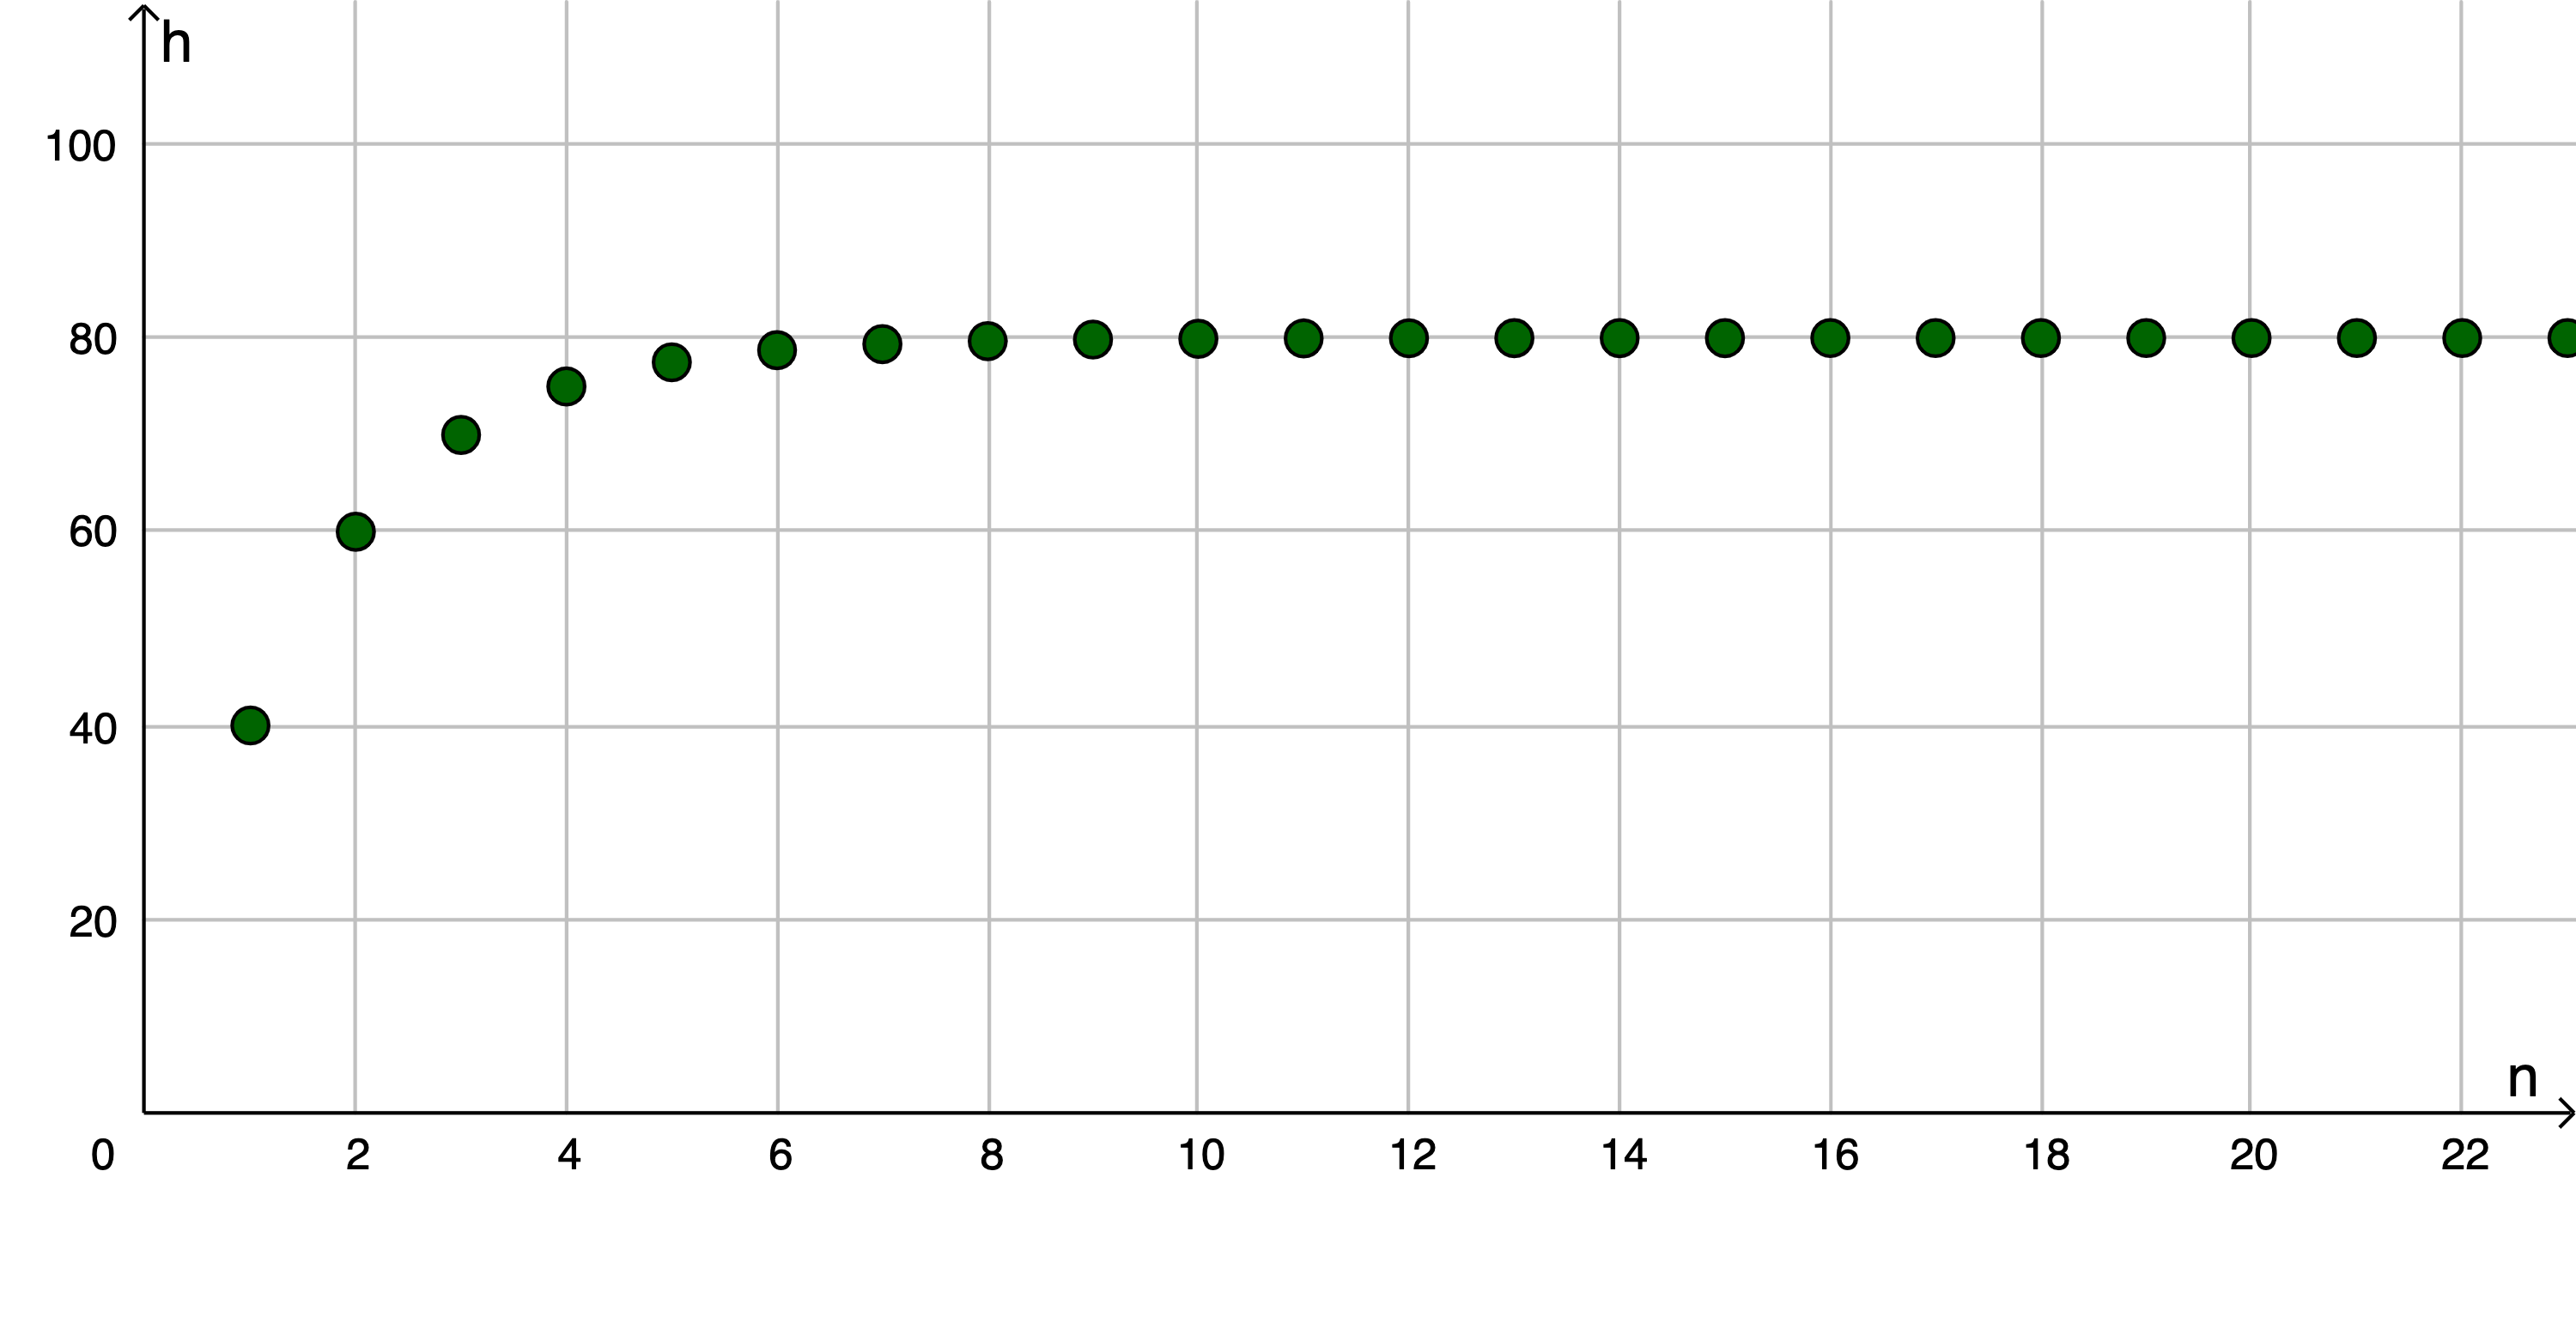
\includegraphics[width=\textwidth]{media/HoeheDerTuerme.png}
	\end{minipage}
	\hfill
	\begin{minipage}{0.3\textwidth}

	\end{minipage}
\end{figure}


% 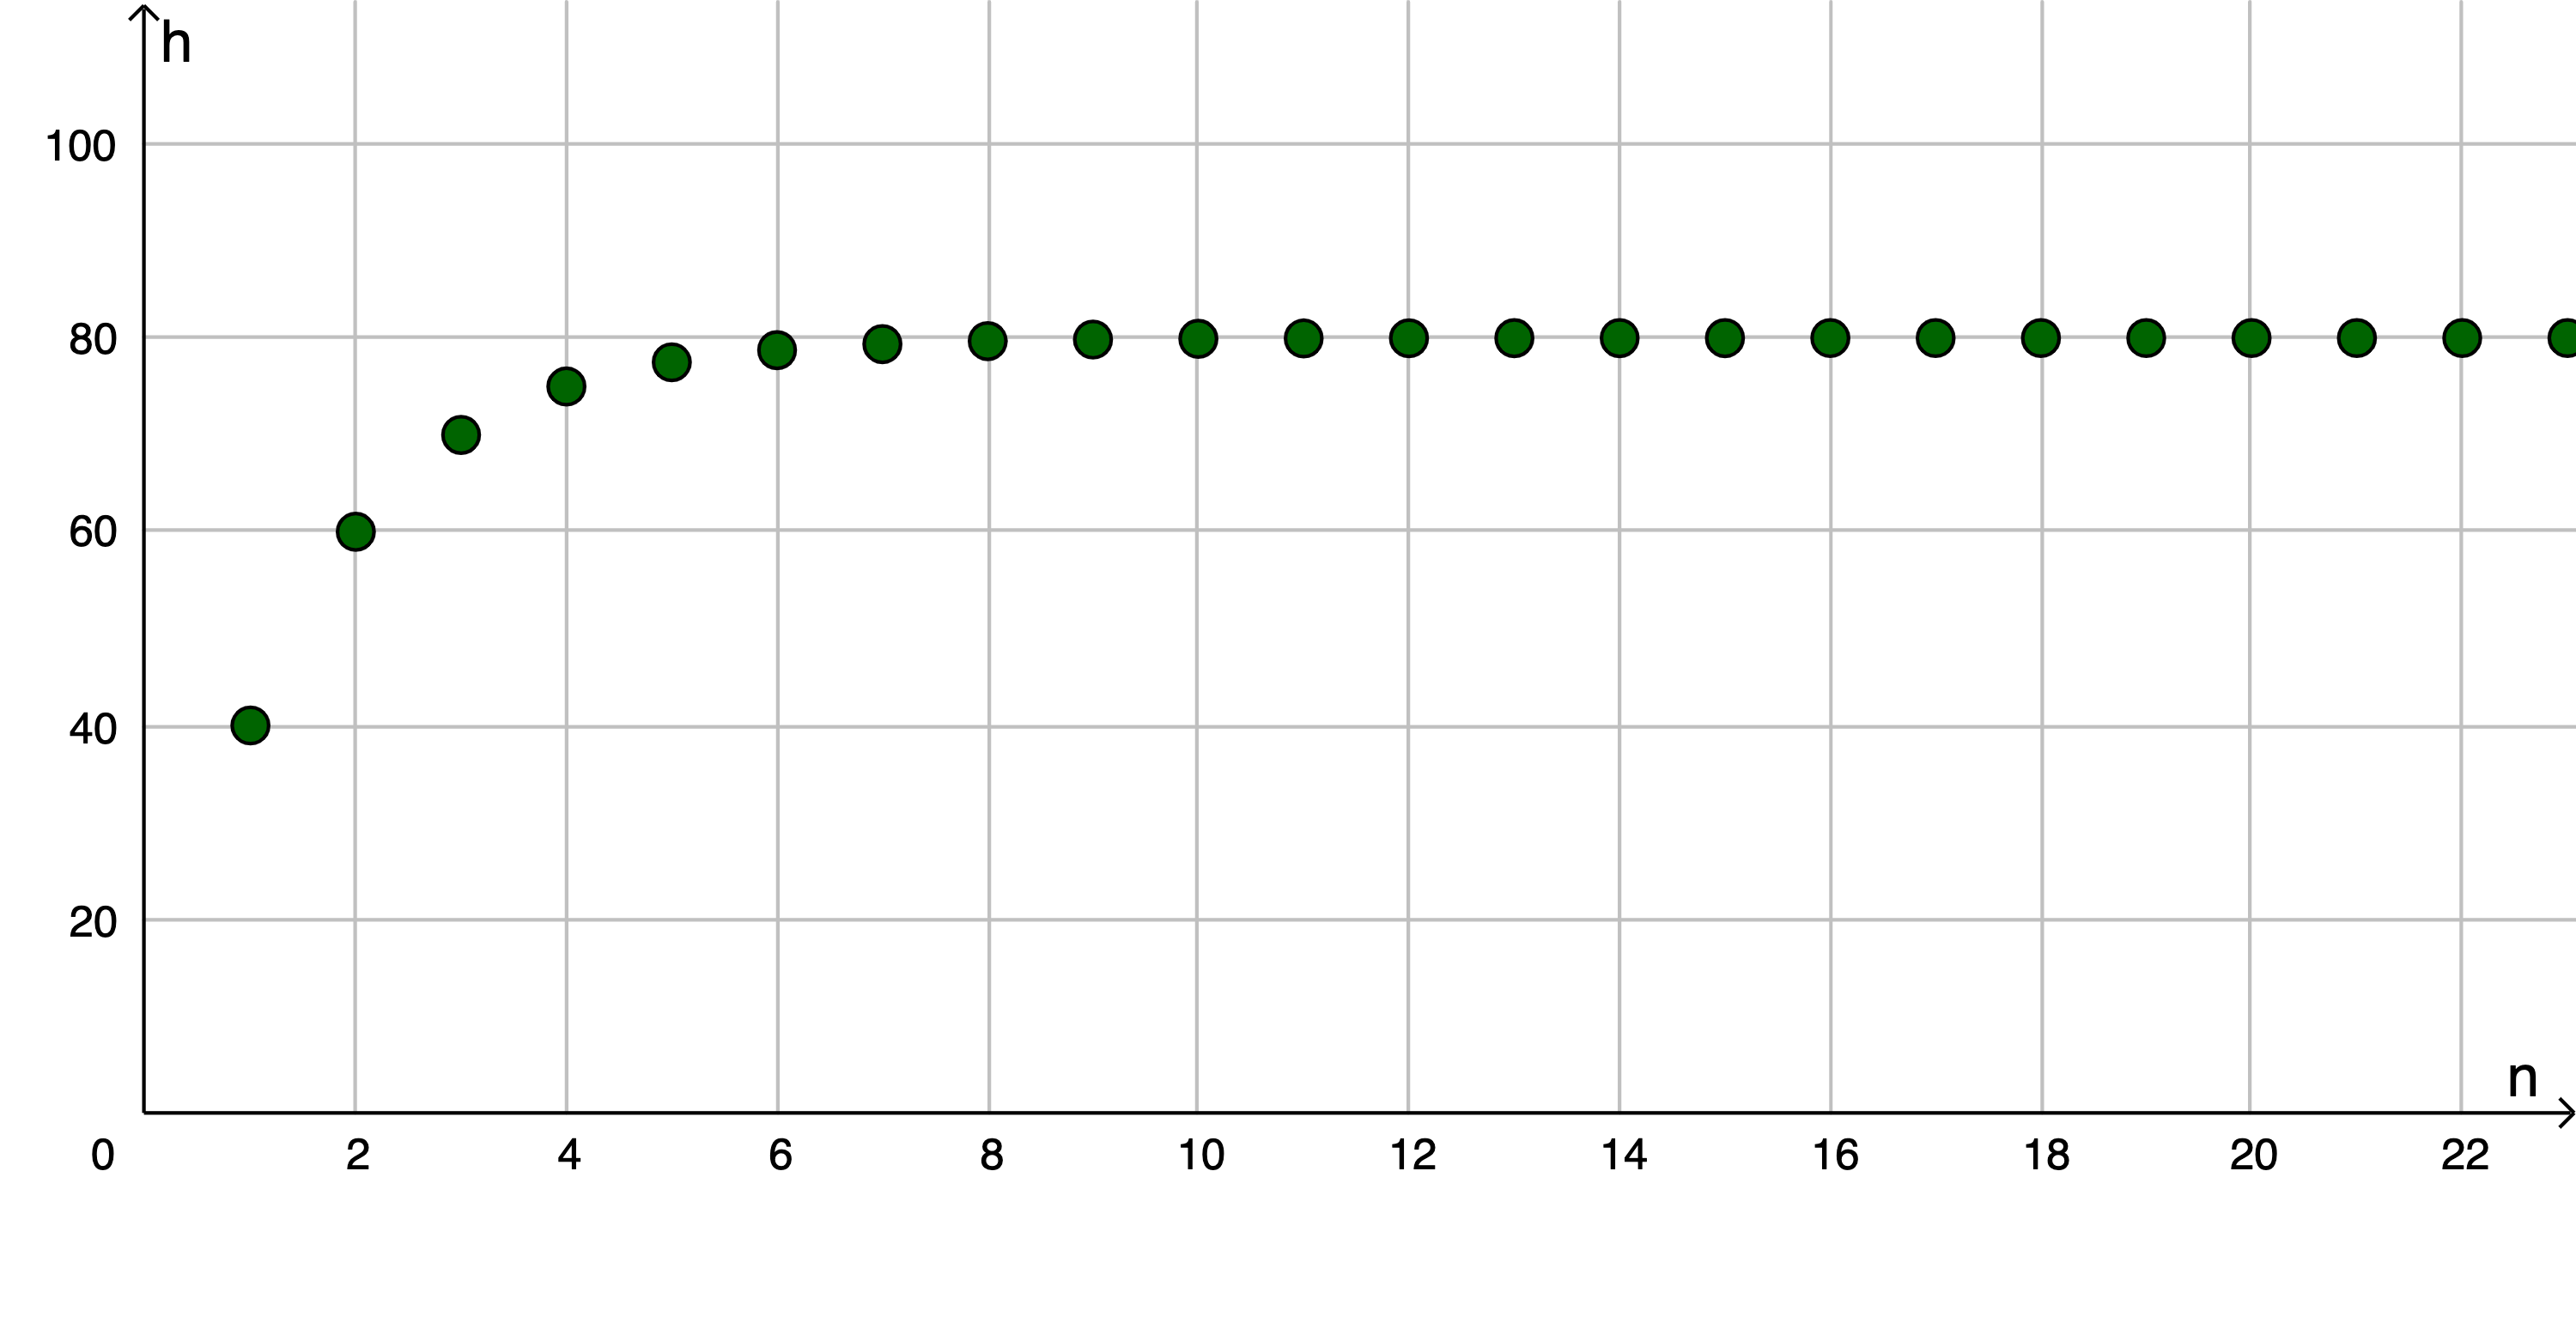
\includegraphics[scale=0.5]{media/HoeheDerTuerme.png} \newline
% \emph{Wieso ist der Grenzwert nicht 100?}
%Die Folgenglieder nähern zwar auch der Zahl 100 immer mehr, aber der Abstand zwischen Folgenglied und 100 ist immer grösser als 20. Erkenntnis: Jeder noch so kleine Abstand zwischen Folgenglieder und vermeintlichen Grenzwert muss unterschritten werden!
%\clearpage
\emph{Wieso ist der Grenzwert nicht 80?}
\begin{figure}[htbp]
	\begin{minipage}{0.5\textwidth}
		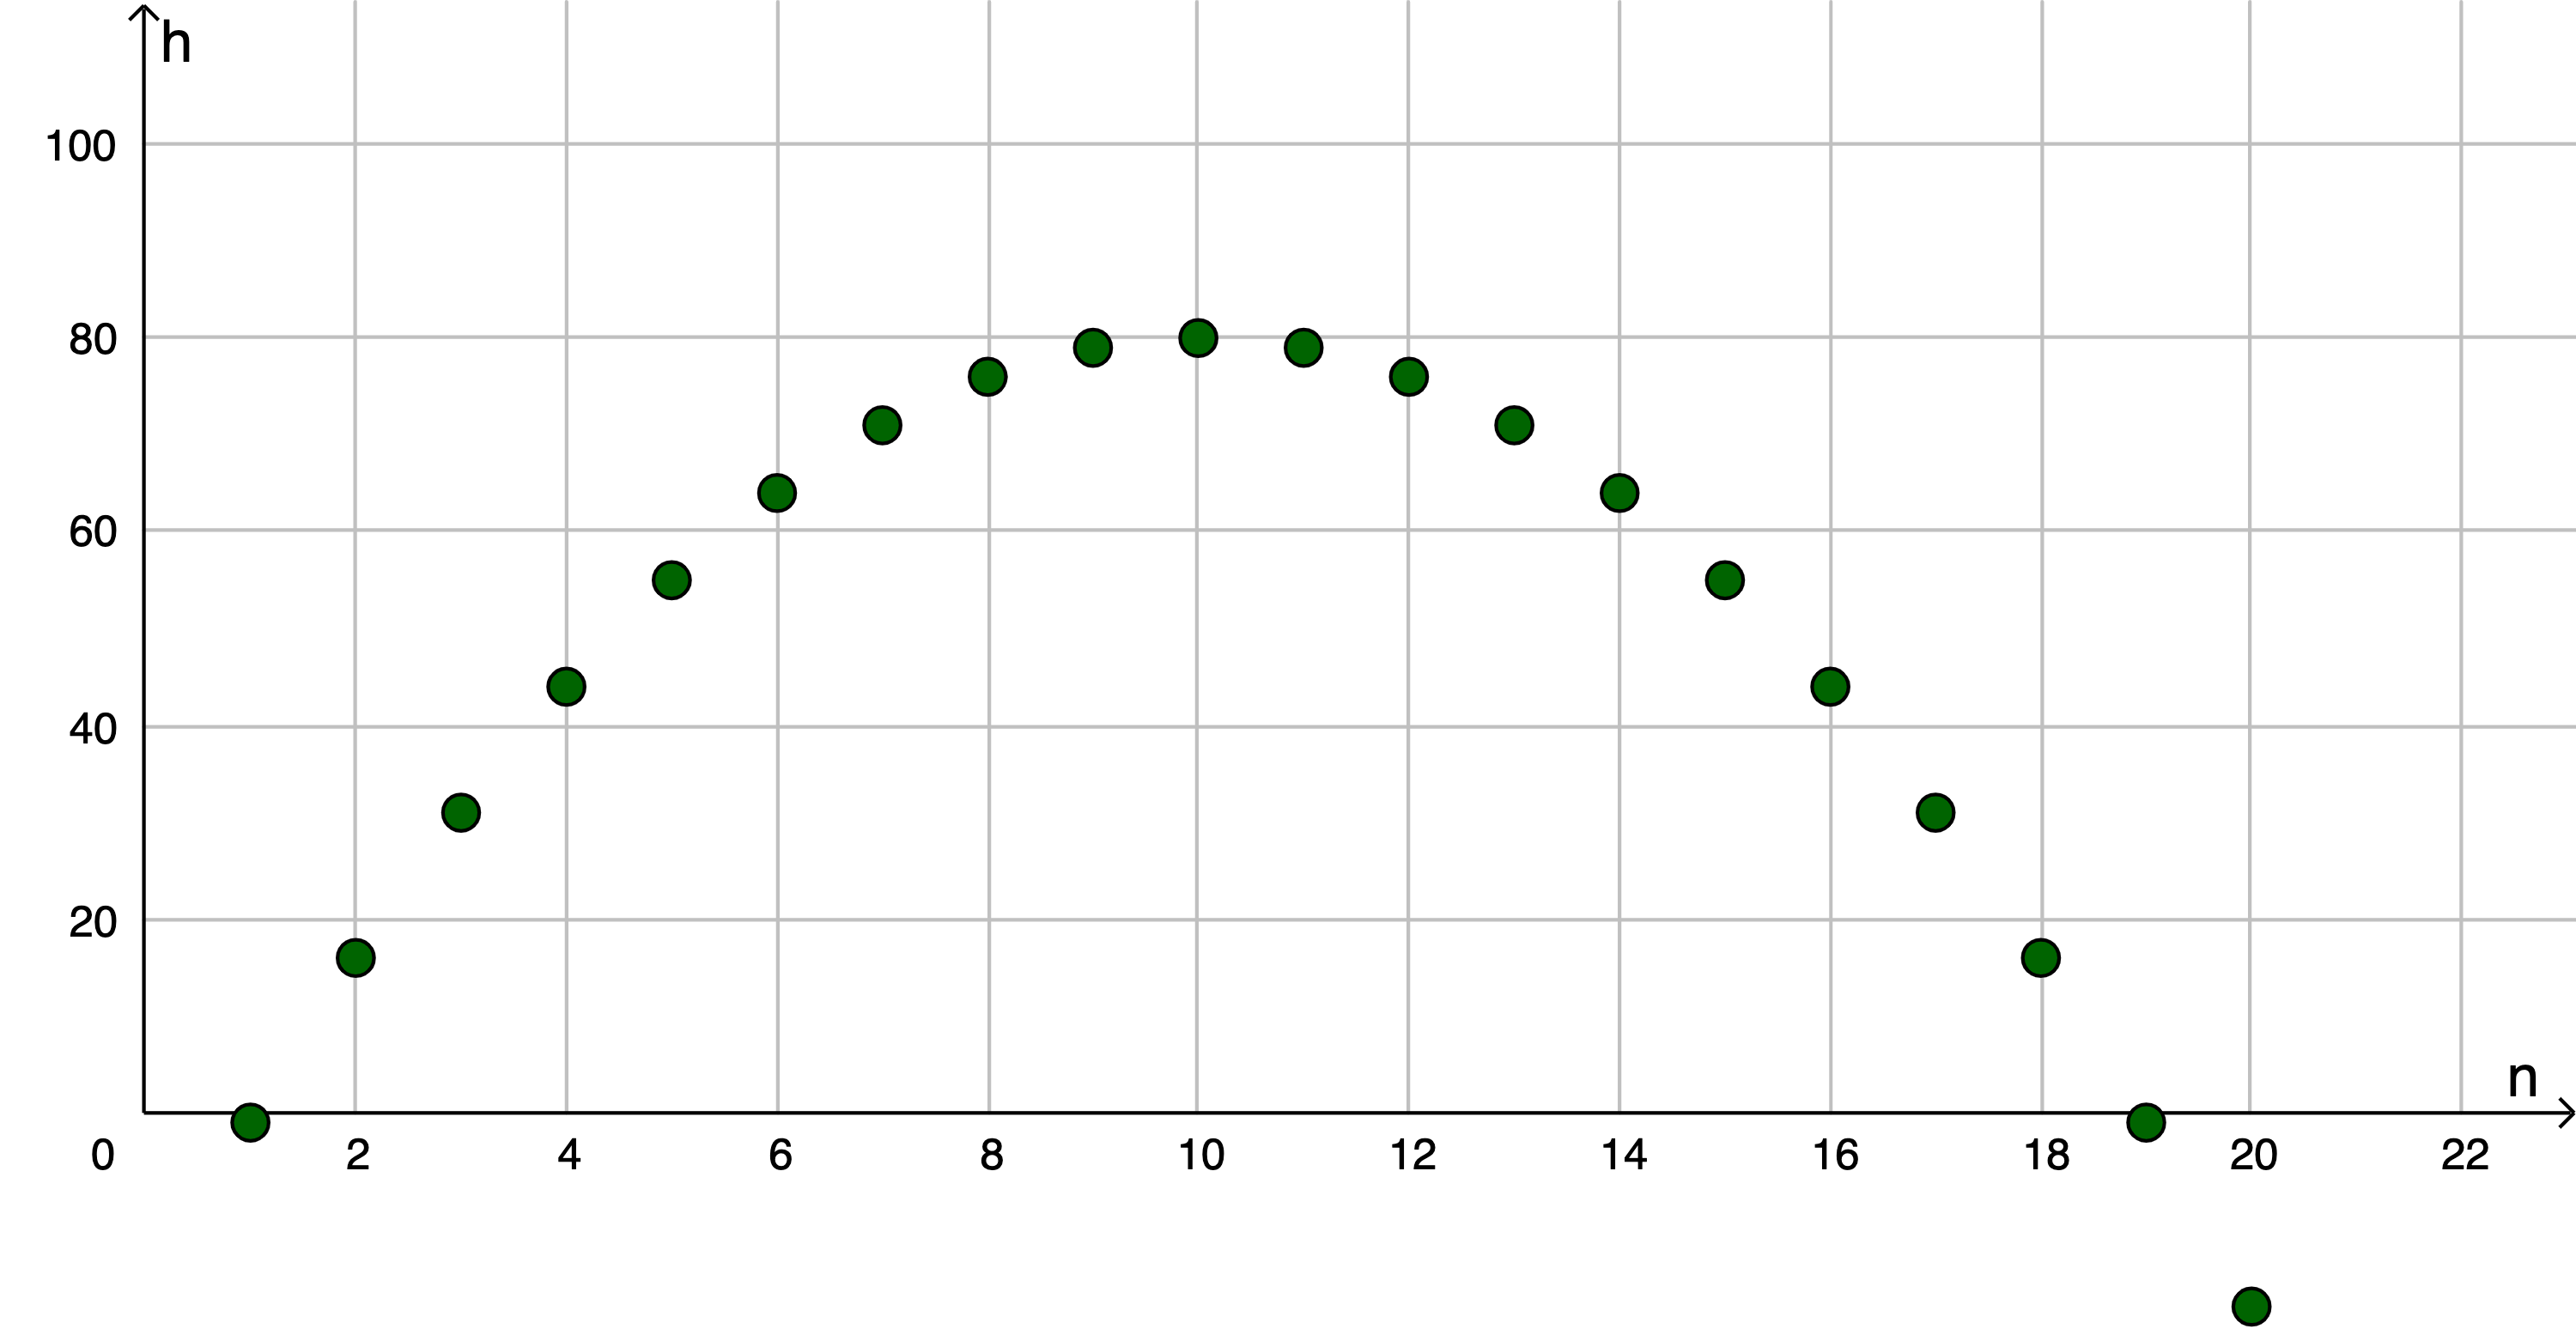
\includegraphics[width=\textwidth]{media/WiesoNicht80.png}
	\end{minipage}
	\hfill
	\begin{minipage}{0.3\textwidth}

	\end{minipage}
\end{figure}
% 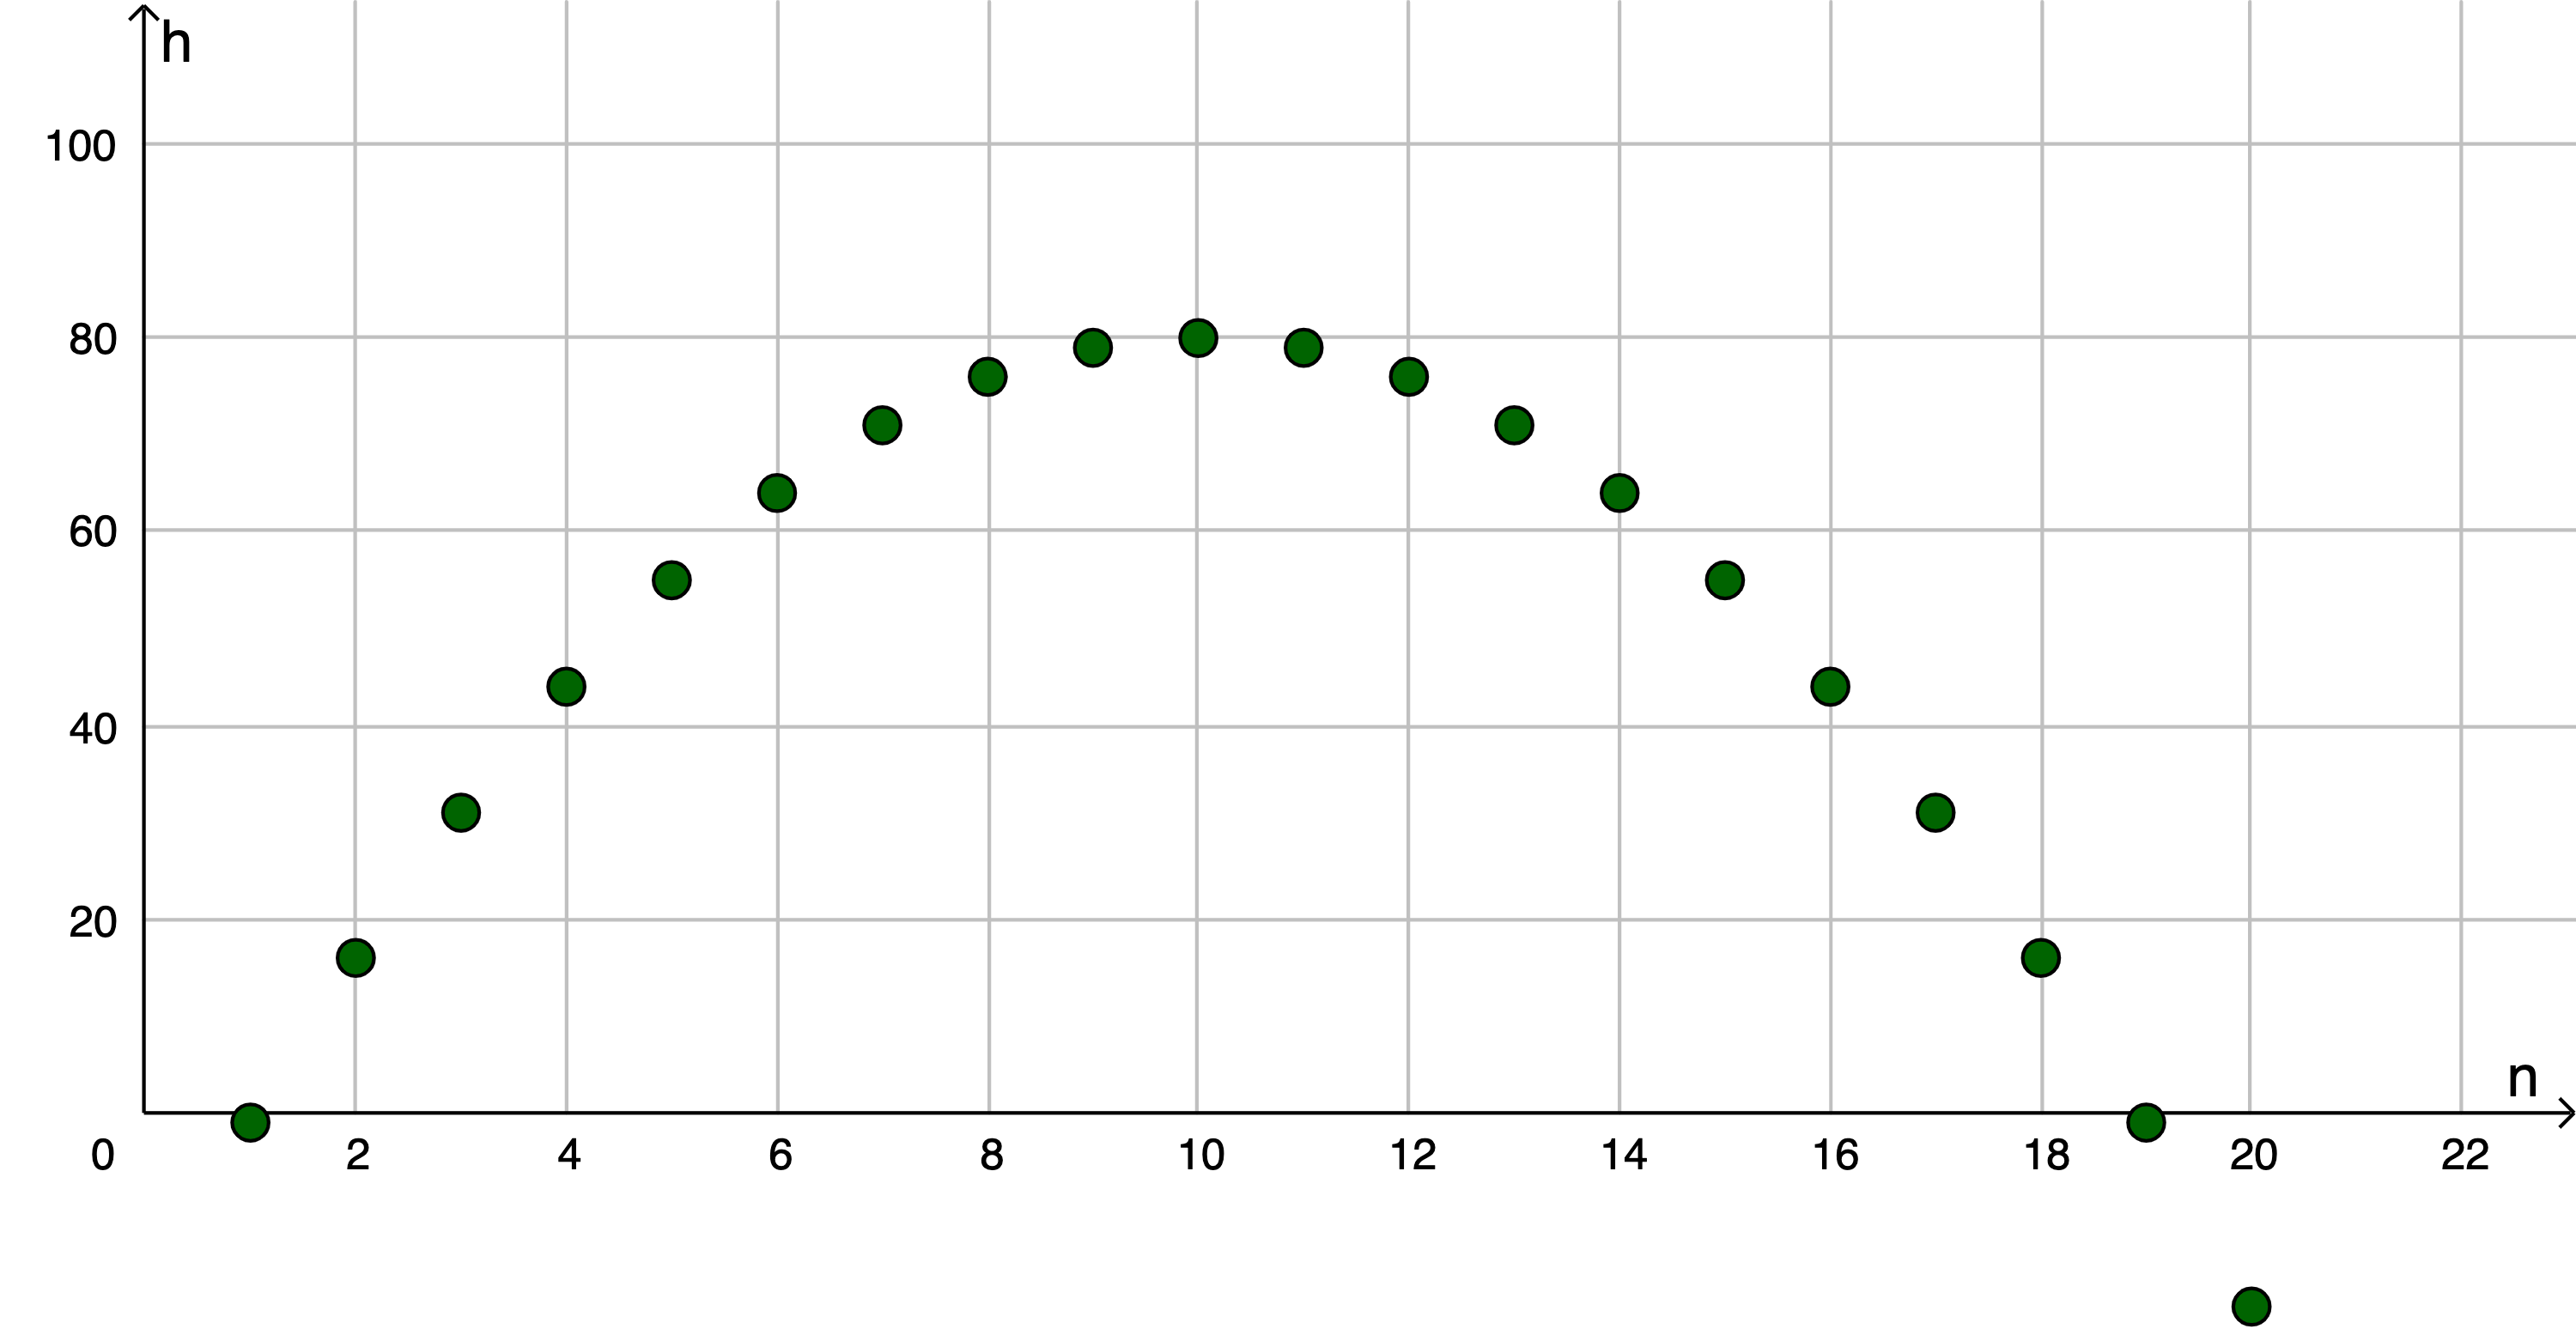
\includegraphics[scale=0.5]{media/WiesoNicht80.png}\newline
% \emph{Wieso ist der Grenzwert nicht 80?}
%Das 10. Glied der Folge im Bild oben ist tatsächlich genau 80. Aber die weiteren Folgenglieder entfernen sich wieder von 80. Erkenntnis: Der Abstand zwischen Folgenglieder und vermeintlichem Grenzwert darf nicht wieder grösser werden!
\clearpage
\begin{definition}{Grenzwert einer Folge}{}
	Eine Zahl $g$ heisst Grenzwert der Folge $a_n$, falls es für jeden noch so kleinen Abstand $\varepsilon>0$ einen Schwellwert $N$ gibt, sodass ab dem $N$-ten Glied der Folge alle Glieder sich um weniger als $\varepsilon$ von $g$ unterscheiden.\newline
	In der Mathematik wird das häufig so angegeben: \newline
	Eine Zahl $g$ heisst Grenzwert der Folge $a_n$, falls: Für alle $\varepsilon>0$ ein $N \in \N$ existiert, sodass für alle $n>N$ gilt
	$$ |a_n - g| < \varepsilon $$
\end{definition}
Anders gesagt: Für jedes (noch so kleine) $\varepsilon > 0$ gibt es eine Schwelle, ab welcher sich alle Folgenglieder in einem \glqq $\varepsilon$-Band\grqq{} um den Grenzwert befinden - also im Bereich Grenzwert$\pm \varepsilon$.

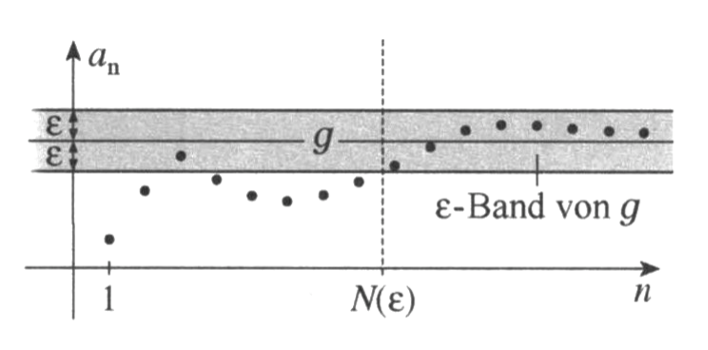
\includegraphics{media/epsilonband.png}

Sprech- und Schreibweisen rund um den Grenzwert:
\begin{itemize}
	\item \glqq Die Folge $a_n$ \emph{konvergiert}\grqq{}.
	\item \glqq Die Folge $a_n$ \emph{strebt} gegen den Grenzwert $g$\grqq{}.
	\item $\lim\limits_{n\rightarrow\infty} a_n = g$ \glqq Der Limes der Folge $a_n$ für $n$ gegen unendlich ist $g$\grqq{}.
	\item $a_n \rightarrow g$ für $n\rightarrow \infty$.
\end{itemize}

Nicht alle Folgen haben einen Grenzwert. Zwei Beispiele für Folgen, die nicht konvergieren:

\begin{figure}[htbp]
	\begin{minipage}{0.5\textwidth}
		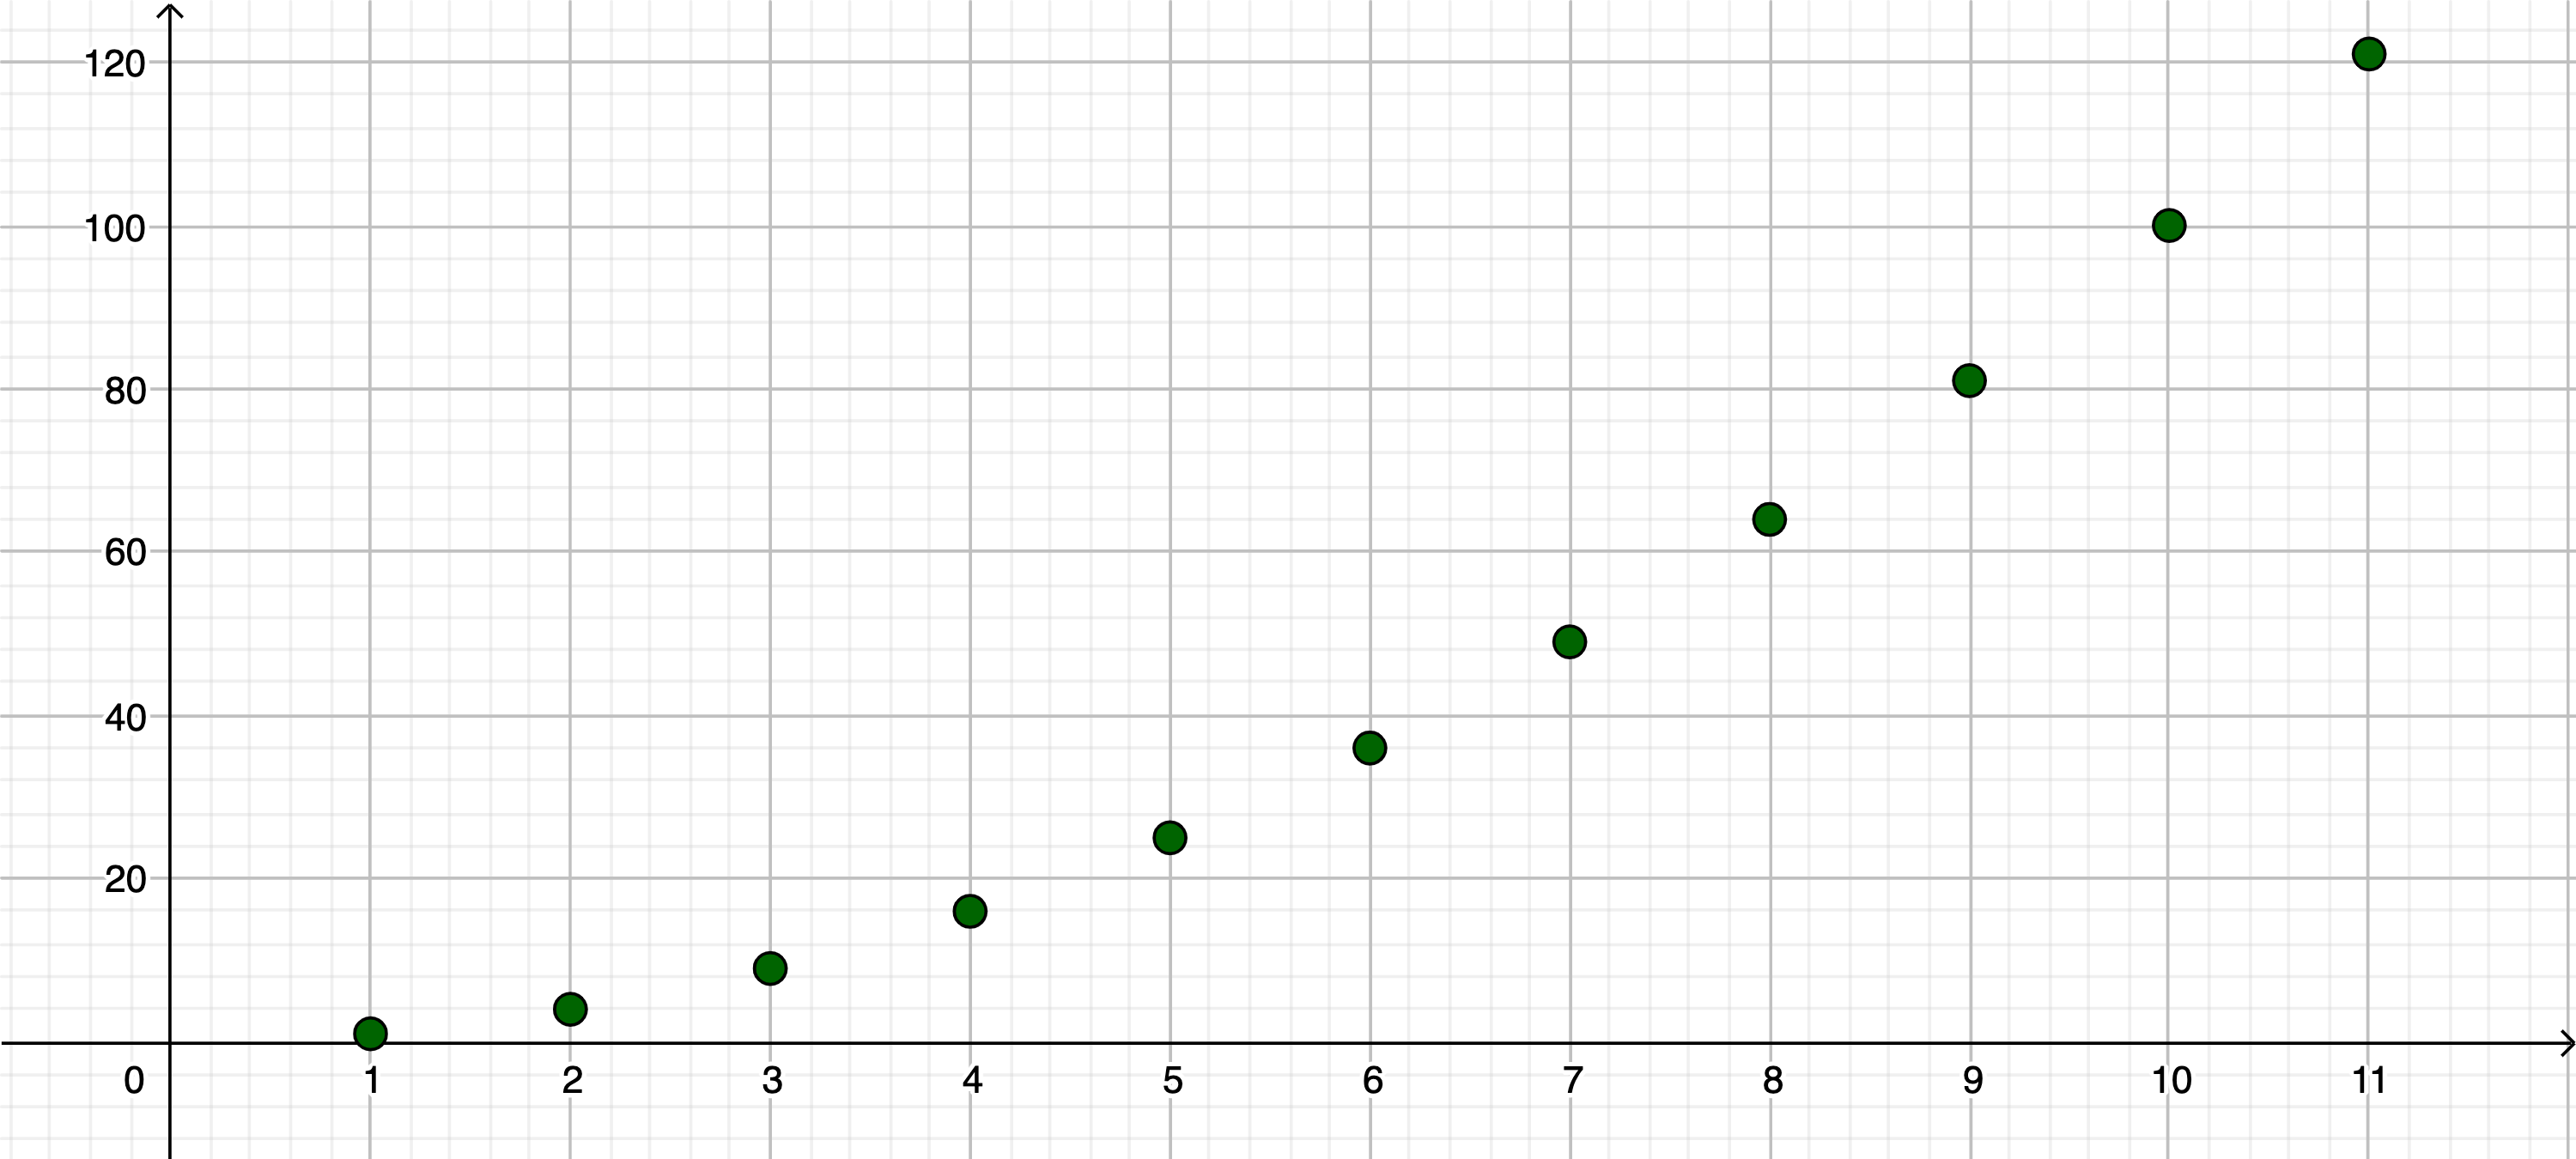
\includegraphics[width=\textwidth]{media/folgeQuadratzahlen.png}
	\end{minipage}
	\hfill
	\begin{minipage}{0.4\textwidth}
		Das Bild zeigt die Folge der Quadratzahlen. Die Glieder dieser Folge wachsen über alle Grenzen. Man sagt: \glqq Die Folge ist divergent\grqq{}. Weil in diesem Fall die Glieder \glqq unendlich gross werden\grqq{}, sagt man auch \glqq die Folge hat den uneigentlichen Grenzwert $\infty$\grqq{} und schreibt $\lim\limits_{n\rightarrow\infty} a_n = \infty$
	\end{minipage}
\end{figure}

\begin{figure}[ht]
	\begin{minipage}{0.5\textwidth}
		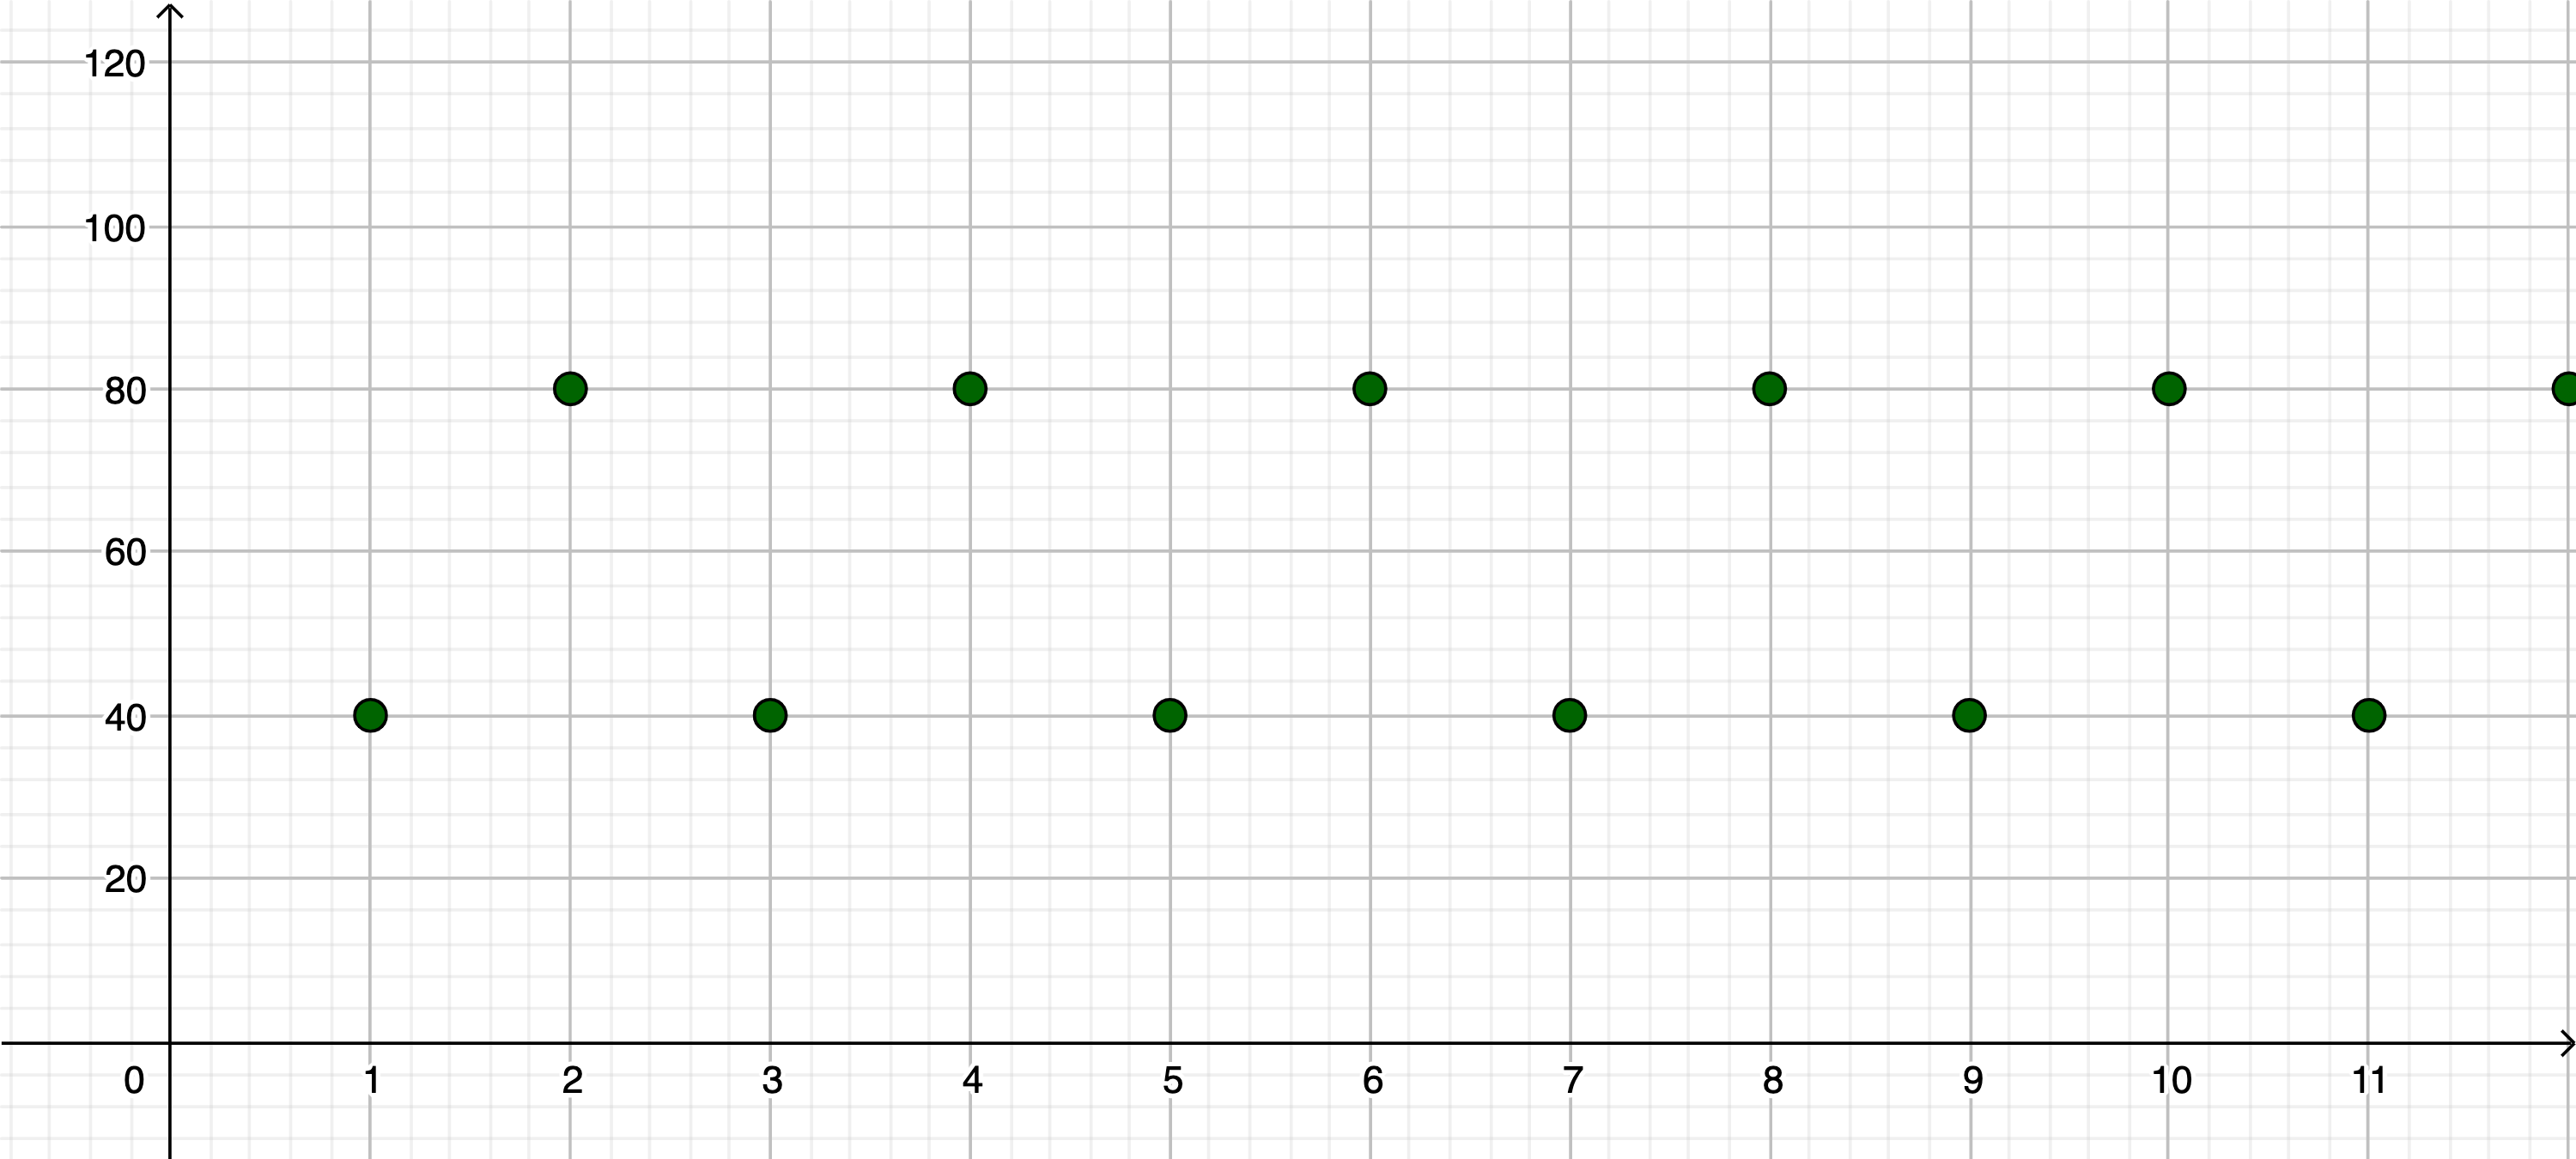
\includegraphics[width=\textwidth]{media/folgeAlternierend.png}
	\end{minipage}
	\hfill
	\begin{minipage}{0.4\textwidth}
		Die Folge in diesem Bild wächst zwar nicht über alle Grenzen, hat aber auch keinen Grenzwert. Sie ist divergent. Der $\lim\limits_{n\rightarrow\infty} a_n$ existiert nicht.
	\end{minipage}
\end{figure}



\begin{bsp}[unbreakable]{Untersuchung der Folge $a_n=\frac{2}{n^2}$}{}

	%\vspace*{16cm}
	Die ersten Glieder der Folge $a_n=\frac{2}{n^2}$ sind: $2, 0.5, 0.2\bar{2}, 0.125, 0.08, 0.05\bar{5}, ...$.
	\bigskip

	\emph{Behauptung}: Die Folge $a_n=\frac{2}{n^2}$  strebt gegen den Grenzwert Null.
	\begin{proof}
		Sei $\varepsilon>0$ eine beliebige (noch so kleine) positive Zahl. Sei dann $N=\sqrt{\frac{2}{\varepsilon}}$ . Nun gilt für alle $n>N$:
		$$ |a_n-0|=|a_n | = \left| \frac{2}{n^2} \right| < \left| \frac{2}{N^2} \right| = \left| \frac{2}{\frac{2}{\varepsilon}} \right| = |\varepsilon| = \varepsilon$$

	\end{proof}
\end{bsp}

Genau gleich kann man allgemein zeigen:
\begin{satz}{Nullfolgen}{}
	Sei $a_n =\frac{c}{n^k}$  mit $k>0$ und $c\in \R$. Dann gilt:
	$$\lim_{n \rightarrow \infty} a_n = 0$$
\end{satz}
\clearpage
\begin{bsp}
	{Schwelle zu gegebener $\varepsilon$-Umgebung bestimmen}{}
	Gegeben ist die Folge $a_n = \frac{2n}{n+1}$. Der Grenzwert der Folge ist $g=2$. Laut Definition gibt es für alle $\varepsilon>0$ eine Zahl $N\in \N$, sodass für alle $n>N$:  $|a_n-g|<\varepsilon$ ist. Bestimmen Sie die kleinstmögliche Zahl $N$ für $\varepsilon= \frac{1}{100}$.
	\vspace*{14cm}
\end{bsp}
\clearpage
\begin{ueb}{}{}
	\begin{enumerate}
		\item
		      Untersuchen Sie die Folge $n \mapsto a_n$. Was vermuten Sie: Ist sie konvergent oder divergent? Was ist der vermutete Grenzwert bzw. die Art der Divergenz an.

		      \begin{enumerate}
			      \item $a_n = \frac{2}{n+2}$
			      \item $a_n = \frac{2n}{n+2}$
			      \item $a_n = \frac{2^n}{n+2}$
			      \item $a_n = \frac{2n + (-1)^n}{n}$
			      \item $a_n = \frac{2 + n \cdot (-1)^n}{n}$
			      \item $a_n = 3 - n \cdot (-1)^n$
			      \item $a_n = \left(1 - \frac{1}{n}\right)^4$
			      \item $a_n = \left(1 - \frac{1}{4}\right)^n$
			      \item $a_n = 2^{-1/n}$
			      \item $a_n = \cos(n\cdot \pi)$
			      \item $a_n = \sin(n\cdot \pi)$
		      \end{enumerate}



		\item Bestimme den Grenzwert $g$ der Folge. Von welchem $n$ an liegen alle Glieder innerhalb der gegebenen $\varepsilon$-Umgebung von $g$?

		      \begin{enumerate}
			      \item $a_n = \frac{1}{2n - 5}, \quad \varepsilon = 0.1$
			            %\item $a_n = \frac{50}{n^2}, \quad \varepsilon = 0.05$
			      \item $a_n = \frac{n - 1}{n + 5}, \quad \varepsilon = 0.02$
			            %\item $a_n = \frac{3n}{n + 4}, \quad \varepsilon = 0.01$
			      \item $a_n = \frac{8}{2^{n-2}}, \quad \varepsilon = 0.0001$
			            %\item $a_n = \frac{2 - 3n^2}{n^2}, \quad \varepsilon = 0.001$
		      \end{enumerate}
	\end{enumerate}
\end{ueb}

\clearpage
\emph{Lösungen}
\begin{enumerate}
	\item \begin{enumerate}
		      \item $a_n = \frac{2}{n+2}$, \quad Grenzwert: $0$
		      \item $a_n = \frac{2n}{n+2}$, \quad Grenzwert: $2$
		      \item $a_n = \frac{2^n}{n+2}$, \quad divergiert gegen $\infty$
		      \item $a_n = \frac{2n + (-1)^n}{n}$, \quad Grenzwert: $2$
		      \item $a_n = \frac{2 + n \cdot (-1)^n}{n}$, \quad unbestimmt divergent
		      \item $a_n = 3 - n \cdot (-1)^n$, \quad unbestimmt divergent ($\pm \infty$)
		      \item $a_n = \left(1 - \frac{1}{n}\right)^4$, \quad Grenzwert: $1$
		      \item $a_n = \left(1 - \frac{1}{4}\right)^n$, \quad Grenzwert: $0$
		      \item $a_n = 2^{-1/n}$, \quad Grenzwert: $1$
		      \item $a_n = \cos(n\cdot \pi)$, \quad unbestimmt divergent
		      \item $a_n = \sin(n\cdot \pi)$, \quad Grenzwert: $0$
	      \end{enumerate}

	\item
	      \begin{enumerate}
		      \item $a_n = \frac{1}{2n - 5}, \quad \varepsilon = 0.1$, \quad Grenzwert: $0$, ab $n \geq 8$
		            %\item $a_n = \frac{50}{n^2}, \quad \varepsilon = 0.05$, \quad Grenzwert: $0$, ab $n \geq 32$
		      \item $a_n = \frac{n - 1}{n + 5}, \quad \varepsilon = 0.02$, \quad Grenzwert: $1$, ab $n \geq 296$
		            %\item $a_n = \frac{3n}{n + 4}, \quad \varepsilon = 0.01$, \quad Grenzwert: $3$, ab $n \geq 1197$
		      \item $a_n = \frac{8}{2^{n-2}}, \quad \varepsilon = 0.0001$, \quad Grenzwert: $0$, ab $n \geq 19$
		            %\item $a_n = \frac{2 - 3n^2}{n^2}, \quad \varepsilon = 0.001$, \quad Grenzwert: $-3$, ab $n \geq 45$
	      \end{enumerate}



\end{enumerate}


























\newpage
\subsubsection{Die Grenzwertsätze}
Das Bestimmen des Grenzwertes und der Nachweis der Konvergenz mit der Definition kann ziemlich aufwendig sein. Einfacher geht es mit den sogenannten Grenzwertsätzen:
\begin{LA}{Einführungsaufgabe}{}
	Betrachten Sie die Folge $a_n=\frac{9n^2+4}{3n^2}$
	\begin{enumerate}
		\item Berechnen Sie $a_1,a_5$ und $a_{10}$.
		\item Welchen Grenzwert hat die Folge vermutlich?
	\end{enumerate}
	Wenn man sehr grosse Zahlen für $n$ einsetzt, kann man leicht eine Vermutung für den Grenzwert der Folge aufstellen. Allerdings kann man nicht ausschliessen, dass man für wirklich sehr grosse $n$ (z.B. $n=10^{{10^9}}$) ganz andere Zahlen erhalten würde; nicht zuletzt deshalb, weil es keinen Computer gibt, der zuverlässig mit solch grossen Zahlen rechnen kann – und es gibt noch viel, viel grössere Zahlen! Durch geschicktes Umformen der Definition der Folge können wir unsere Vermutung aber begründen:
	\begin{enumerate}
		\item Die Definition der Folge $a_n$ kann auch so umgeformt werden:
		      $$a_n=\frac{9n^2}{3n^2}+\frac{4}{3n^2}=3 + \frac{4}{3n^2}$$
		      Was passiert mit den Summanden in der Definition der Folge, wenn $n$ immer grösser wird? Was bedeutet das für den Grenzwert?
		\item Bestimmen Sie den Grenzwert der Folge $b_n=\frac{2n+10}{5n}$, indem Sie den Term zuerst umformen.
		\item Wie lautet der Grenzwert der Folge $c_n= \frac{9n^2+4}{3n^2} + \frac{2n+10}{5n}$?
	\end{enumerate}
\end{LA}
\newpage
In den Einführungsaufgaben haben Sie implizit die sogenannten Grenzwertsätze verwendet:
\begin{satz}{Grenzwertsätze}{}
	Sind die Folgen $a_n$ und $b_n$ konvergent, so sind es auch die Folgen $a_n\pm b_n, a_n\cdot b_n$ und, sofern $b_n\neq 0$ und $\lim_{n\rightarrow \infty} b_n \neq 0$, auch die Folge $\frac{a_n}{b_n}$. Für die Grenzwerte gilt
	$$\lim_{n\rightarrow \infty} \left(a_n \pm b_n \right) = \lim_{n\rightarrow \infty} a_n \pm \lim_{n\rightarrow \infty} b_n $$
	$$\lim_{n\rightarrow \infty} \left(a_n \cdot b_n \right) = \lim_{n\rightarrow \infty} a_n \cdot \lim_{n\rightarrow \infty} b_n $$
	$$\lim_{n\rightarrow \infty} \left( \frac{a_n}{b_n} \right) = \frac{\lim_{n\rightarrow \infty} a_n}{\lim_{n\rightarrow \infty} b_n}$$
\end{satz}
Damit lassen sich viele Grenzwerte einfach berechnen:
\begin{bsp}{Anwendung der Grenzwertsätze}{}
	\begin{enumerate}
		\item $a_n=\frac{4n^2-17}{3n^2+n}$ Grenzwert? \vspace{3.5cm}
		\item $b_n=\frac{5n^3-n^2+2}{-2n^2+n-2}$ Grenzwert? \vspace{3.5cm}
		\item $c_n=\frac{n^2+2}{n^4+n-3}$ Grenzwert? \vspace{3.5cm}
	\end{enumerate}
\end{bsp}

Merke \textbf{HPG}: Bein Grenzwert für $n\to\infty$ gilt: die \glqq \textbf{H}öchste \textbf{P}otenz \textbf{G}ewinnt\grqq.
\clearpage
\begin{ueb}{}{}
	\begin{enumerate}
		\item Bestimme den Grenzwert der Folge $n \mapsto a_n$ mithilfe der Grenzwertsätze.

		      \begin{enumerate}
			      \item $a_n = \frac{4 + \frac{1}{n}}{\frac{2}{n}-1}$
			      \item $a_n = \left(3 + \frac{1}{n}\right)(4 - \frac{1}{n})$
			      \item $a_n = \frac{(n - 3)^2 \cdot n}{n^2 + 1}$
			      \item $a_n = \frac{(3n - 1)^3}{n^3}$
			      \item $a_n = 3 + 0.8^n$
			      \item $a_n = \frac{(2n - 1)(3n + 5)}{(n + 2)(4n - 1)}$
			      \item $a_n = 7 + \frac{4n + 1}{n + 3}$
			      \item $a_n = \frac{\frac{3}{n+1} - \frac{4}{n}}{\frac{1}{n}}$
			      \item $a_n = \frac{(n + 4)^3 - n^3}{(n + 4)^3 + n^3}$
			      \item $a_n = \frac{3^n + 1}{3^{n+1}}$ Tipp: Erweitern Sie mit $\frac{1}{3^n}$
			      \item $a_n = \frac{3^n}{3^n \cdot 3^{-n}}$
			      \item $a_n = \frac{4^{n+1}}{4^n - 4^{n-1}}$
		      \end{enumerate}
		\item Berechne den vom Wert des Parameters $a \in \mathbb{R}$ abhängigen Grenzwert.

		      \begin{enumerate}
			      \item $\lim\limits_{k \to \infty} \frac{a^2 k}{a^2 k - 1}$
			      \item $\lim\limits_{k \to \infty} \frac{a k}{a^2 k + 2}$
		      \end{enumerate}
	\end{enumerate}
\end{ueb}

\clearpage
\emph{Lösungen}
\begin{enumerate}
	\item \begin{enumerate}
		      \item $a_n = \frac{4 + \frac{1}{n}}{ \frac{2}{n}-1}$, \quad Grenzwert: $-4$
		      \item $a_n = \left(3 + \frac{1}{n}\right)(4 - \frac{1}{n})$, \quad Grenzwert: $12$
		      \item $a_n = (n - 3)^2 \cdot\frac{ n}{n^2 + 1}$, \quad Grenzwert: $\infty$
		      \item $a_n = \frac{(3n - 1)^3}{n^3}$, \quad Grenzwert: $27$
		      \item $a_n = 3 + 0.8^n$, \quad Grenzwert: $3$
		      \item $a_n = \frac{(2n - 1)(3n + 5)}{(n + 2)(4n - 1)}$, \quad Grenzwert: $\frac{3}{2} $
		      \item $a_n = 7 + \frac{4n + 1}{n + 3}$, \quad Grenzwert: $11$
		      \item $a_n = \frac{\frac{3}{n+1} - \frac{4}{n}}{\frac{1}{n}}$, \quad Grenzwert: $-1$
		      \item $a_n = \frac{(n + 4)^3 - n^3}{(n + 4)^3 + n^3}$, \quad Grenzwert: $0$
		      \item $a_n = \frac{3^n + 1}{3^{n+1}}$, \quad Grenzwert: $\frac{1}{3}$
		      \item $a_n = \frac{3^n}{3^n \cdot 3^{-n}}$, \quad Grenzwert: $\infty$
		      \item $a_n = \frac{4^{n+1}}{4^n - 4^{n-1}}$, \quad Grenzwert: $\frac{16}{3}$
	      \end{enumerate}

	\item

	      Berechne den vom Wert des Parameters $a \in \mathbb{R}$ abhängigen Grenzwert.

	      \begin{enumerate}
		      \item Falls $a=0$ Grenzwert $0$, andernfalls Grenzwert: $1$
		      \item Falls $a=0$ Grenzwert $0$, andernfalls Grenzwert: $1/a$
	      \end{enumerate}
\end{enumerate}















\newpage
\begin{proof}[Beweis der Grenzwertsätze]
	Stellvertretend für alle anderen, wird im Folgenden der erste Grenzwertsatz bewiesen:

	\emph{Behauptung:} Sind die Folgen $a_n$ und $b_n$ konvergent, so ist es auch die Folge $a_n + b_n$.  Für den Grenzwert gilt
	$$\lim_{n\rightarrow \infty} \left(a_n + b_n \right) = \lim_{n\rightarrow \infty} a_n + \lim_{n\rightarrow \infty} b_n $$
	Sei $\lim_{n\rightarrow \infty} a_n = a$ und $ \lim_{n\rightarrow \infty} b_n = b$.
	Gemäss der Definition der Konvergenz müssen wir zeigen, dass für jede Toleranz $\varepsilon>0$ eine Schwelle $N$ existiert, sodass $|(a_n+b_n )-(a+b)|<\varepsilon$ für alle $n>N$. Mit der Dreiecksungleichung\footnote{Die Dreiecksungleichung besagt, dass für alle Zahlen $x,y$ gilt: $|x+y|\le |x|+|y|$} gilt:
	$$|(a_n+b_n)-(a+b)|\le |a_n - a|+|b_n - b|$$
	Da aber $a_n$ gegen $a$ konvergiert, wird der Term $|a_n-a|$ verschwindend klein. Insbesondere gibt es eine Schwelle $N_a$, sodass $|a_n-a|<\frac{\varepsilon}{2}$ ist, für alle $n>N_a$.\newline
	Analog gibt es eine Schwelle $N_b$, sodass $|b_n-b|<\frac{\varepsilon}{2}$ ist, für alle $n>N_b$. \newline
	Sei nun $N_{ab} = \max \{N_a, N_b\}$. Dann gilt für alle $n>N_{ab}$.
	$$|(a_n+b_n )-(a+b)|\le |a_n-a|+|b_n-b|<\frac{\varepsilon}{2}+\frac{\varepsilon}{2}= \varepsilon$$
	Auf diese Art kann man für jedes (beliebig kleine) $\varepsilon>0$ eine Schwelle $N$ finden, sodass $|(a_n+b_n )-(a+b)|<\varepsilon$ für alle $n>N$. Somit konvergiert $a_n+b_n$ gegen $a+b$.
\end{proof}
